\chapter{Qubit calibration}

In this chapter I will describe the process of calibration for superconducting flux-tunable transmon on the hardware located in the QRC (Quantum Research Center) Laboratory of the TII (Technology \& Innovation Institute) in Abu Dhabi.

\section{Experimental setup}
All the results presented in this work were obtained using the Contralto-D chip \cite{qw11q}, which offers up to 21 fully connected qubits and 4 isolated qubits, for a total of 25 physical qubits.
The distinction between fully connected and isolated qubits is important as only the fully connected subset supports direct two-qubit gate operations, which are essential for implementing entangling gates and complex quantum circuits. 
Isolated qubits, while still operational for single-qubit tasks, do not participate in multi-qubit interactions and thus are not functionally equivalent in terms of computational capabilities.
The topology of the qubit is shown in figure \ref{fig:qw11q_topology}.

\begin{figure}[ht!]
    \centering
    \begin{subfigure}{0.40\textwidth}
        \centering
        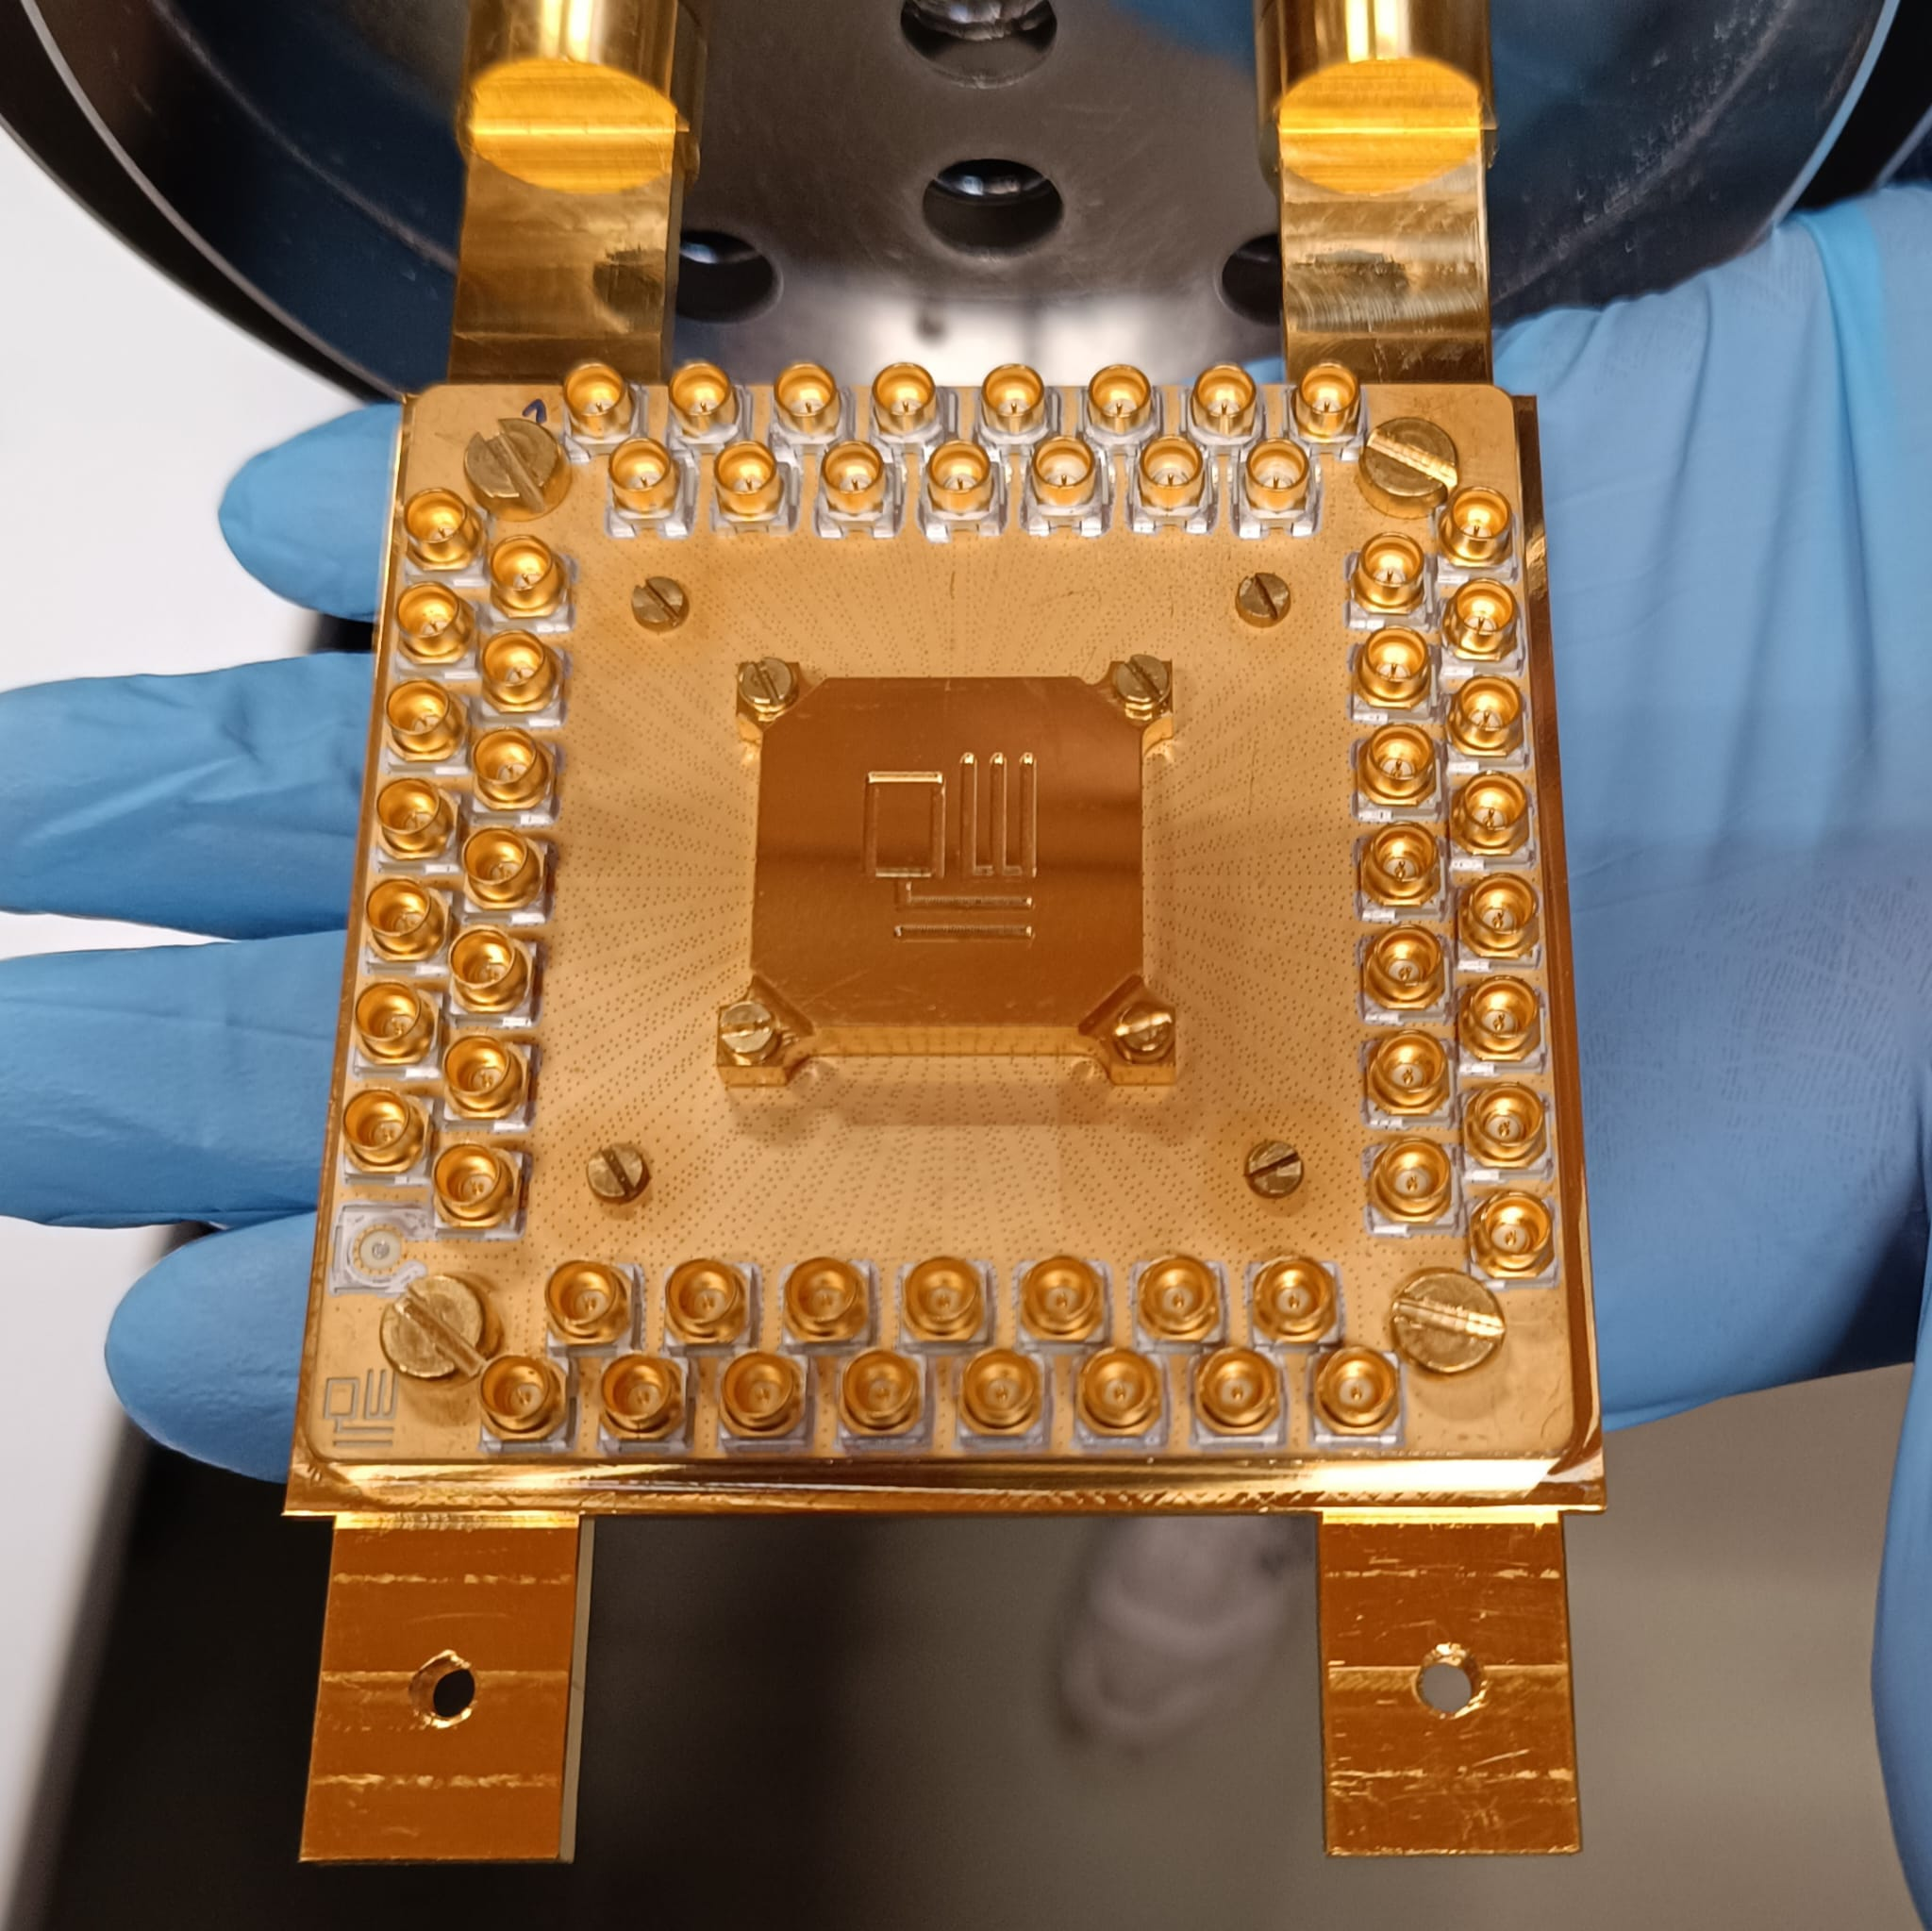
\includegraphics[width=0.80\textwidth]{figures/png/qw11q.jpeg}
        \subcaption{}
        \label{fig:qw11q_picture}
    \end{subfigure}
    \hfill
    \begin{subfigure}{0.50\textwidth}
        \centering
        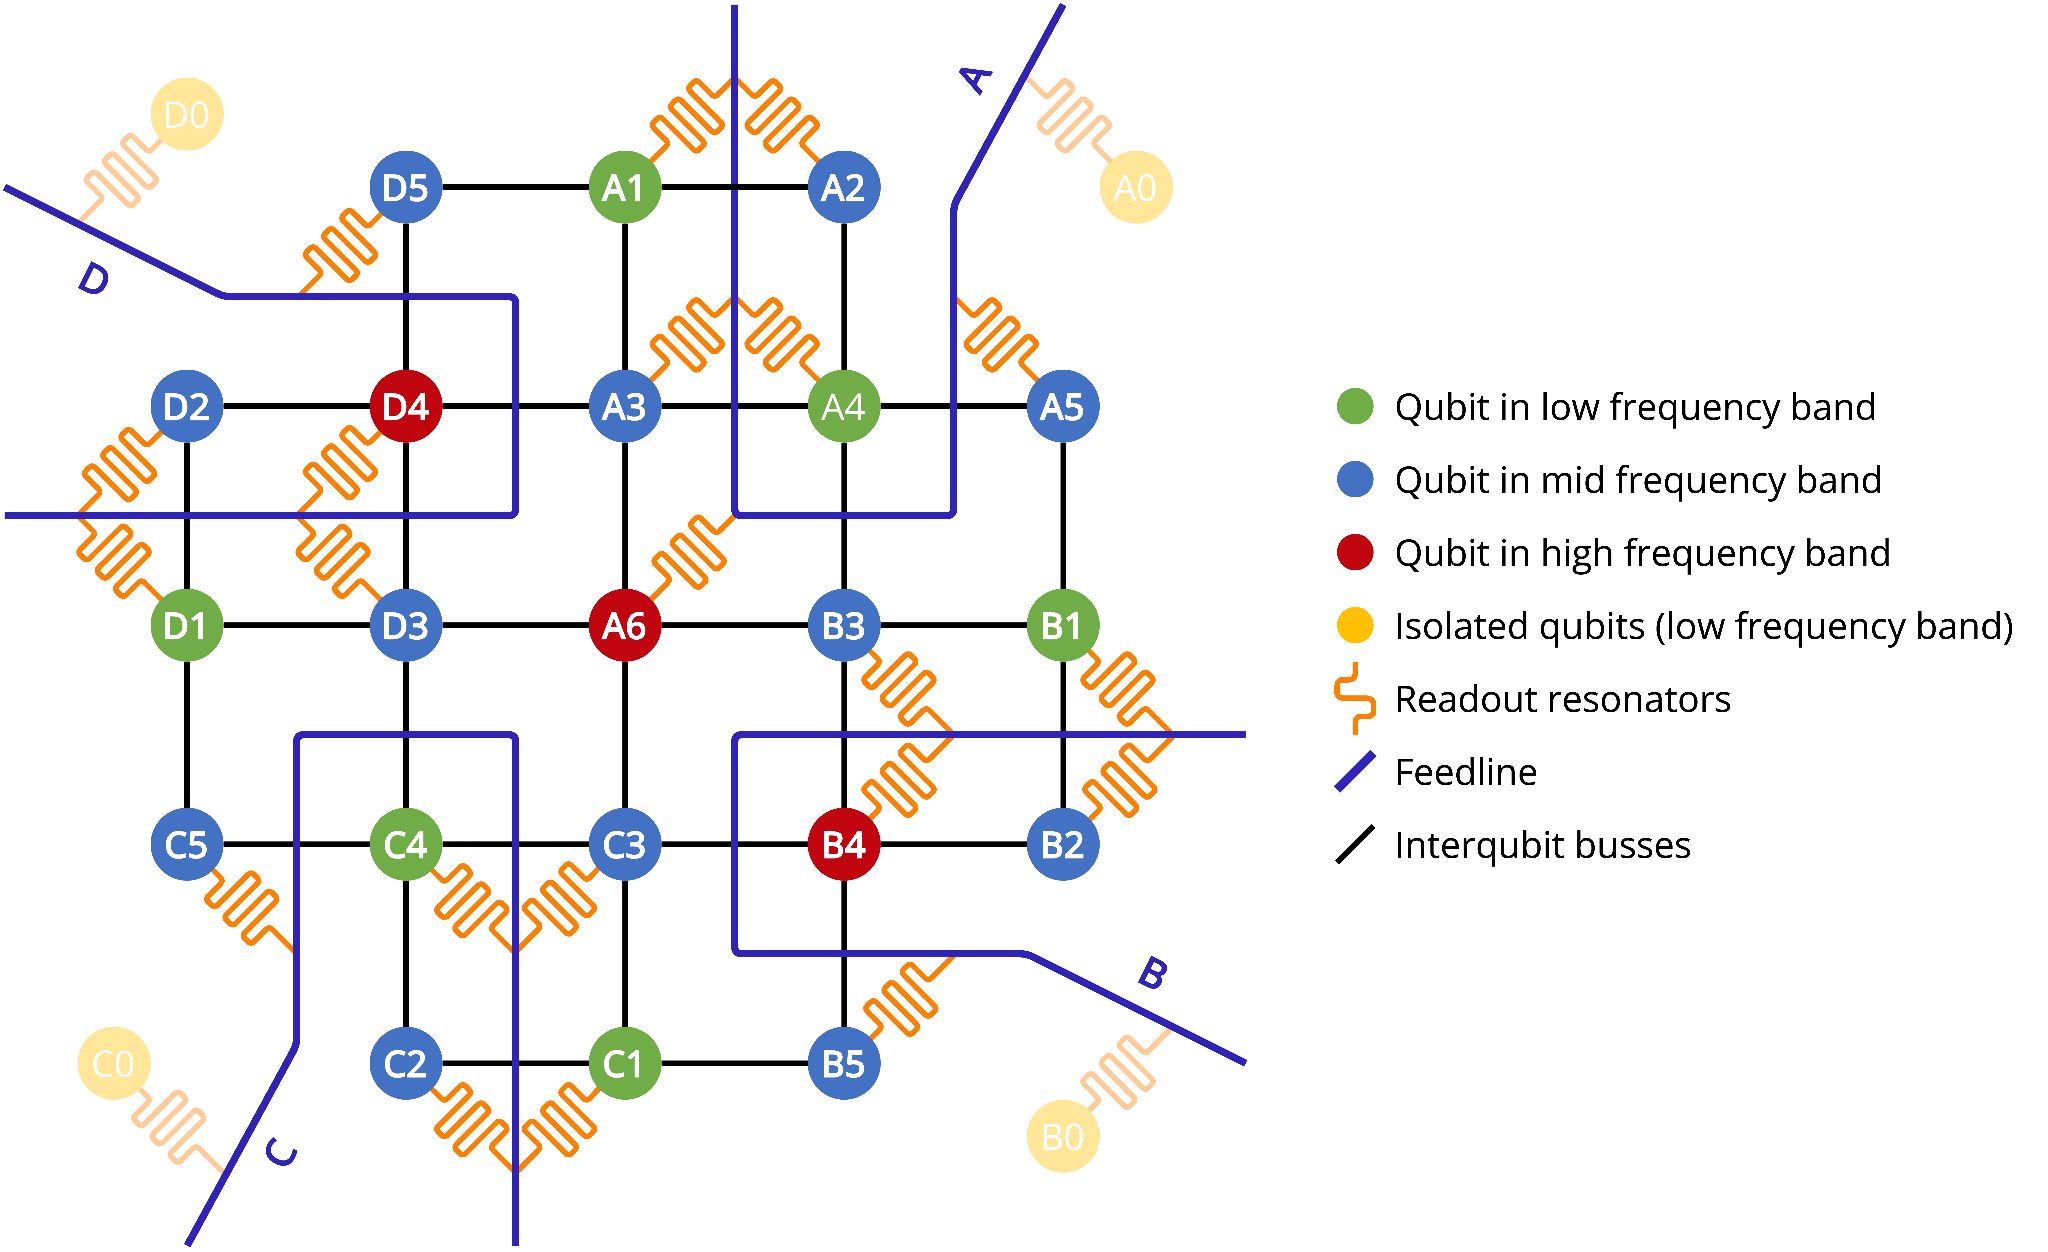
\includegraphics[width=\textwidth]{figures/png/qw11q.png}
        \subcaption{}
        \label{fig:qw11q_topology}
    \end{subfigure}
    \caption{Figure \ref{fig:qw11q_picture}: Picture of the Contralto-D chip from QuantWare. Figure \ref{fig:qw11q_topology}: Topology of the Contralto-D chip from QuantWare.}
    \label{fig:qw11q}
\end{figure}

As discussed in the previous chapter, the behavior of Josephson junctions and SQUIDs relies critically on the superconducting state of the materials involved. 
To achieve and maintain this regime, it is essential that the superconducting elements operate well below their critical temperature. 
For this reason, the Contralto-D chip is installed at the lowest temperature stage of the cryostat, where the required thermal conditions for superconductivity are met. 
This ensures the proper functioning of the quantum hardware and enables the realization of coherent quantum operations.

These systems achieve ultra-low temperatures by exploiting the unique quantum properties of helium-3 (\ce{^{3}He}) and helium-4 (\ce{^{4}He}) isotopes in a dilution process.
At the core of a dilution refrigerator is a mixing chamber, where the cooling mechanism takes place. 
When a mixture of \ce{^{3}He} and \ce{^{4}He} is cooled below approximately 870 millikelvin, the two isotopes phase-separate into a \ce{^{3}He}-rich phase and a \ce{^{3}He}-dilute phase. 
The key principle is that when \ce{^{3}He} atoms cross the phase boundary—from the concentrated phase into the dilute phase—they absorb energy from their surroundings. 
This process is endothermic and is the fundamental source of cooling in the dilution refrigerator.\\
The system operates as a closed loop: \ce{^{3}He} gas is circulated using a combination of sorption pumps and still pumps, which remove \ce{^{3}He} vapor from the still (typically at $600–800 mK$), recondense it at a higher stage, and reintroduce it into the mixing chamber. 
The refrigerator includes several thermalization stages—typically at $50 K$, $4 K$, $800 mK$, $100 mK$, and finally below $20 mK$—each connected to a corresponding cooling stage and separated by radiation shields and thermal filters to minimize heat load and noise from higher-temperature stages.
Dilution refrigerators are highly stable and capable of reaching base temperatures below $10 mK$, with hold times on the order of days or even weeks. 
These temperatures are crucial for achieving the low thermal noise and long coherence times necessary for high-fidelity quantum operations in superconducting circuits.
Specifically the cryostat employed in the lab is the XLDsl from Bluefors \cite{XLD1000}, an image of the cryostat is shown in figure \ref{fig:XLDsl}.

\begin{figure}[h!]
    \centering
    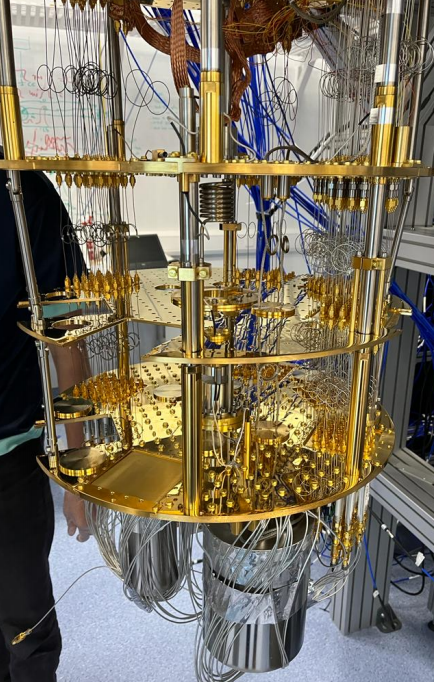
\includegraphics[width=0.35\textwidth]{figures/png/XLD1000.png}
    \caption{Picture of the XLDsl dilution refrigerator at the QRC Lab}
    \label{fig:XLDsl}
\end{figure}

Outside the cryostat, the control and readout of superconducting qubits are managed by dedicated room-temperature electronics.
These systems are responsible for generating the microwave pulses used to drive single- and two-qubit gates, as well as for acquiring and processing the output signals that encode the qubit states 
Typically they include arbitrary waveform generators (AWGs), microwave sources, mixers, digitizers, and field-programmable gate arrays (FPGAs).
The generated microwave pulses are shaped and modulated at room temperature before being attenuated and routed to the cryogenic environment. 
Similarly, signals returning from the qubits are amplified and digitized for state discrimination and further processing. 
The electronics employed in the lab for the control of the \tt{qw11q} is the OPX1000 platform by Quantum Machines \cite{opx1000}.

\section{Calibration experiments}

The first task that I needed to complete at the beginning of my thesis work was the calibration of at least a line of the superconducting quibts of the Contralto-D chip using the \tt{Qibocal} library.
Da qui in avanti per ragioni di brevità indicherò il chip come \tt{qw11q}, il nome del nodo con cui è registrato sul cluster di calcolo del QRC.
In the following I will describe the experiments that I performed and commenting on the results.

\subsection{DRAG experiment}\label{sec:DRAG}
\cite{Motzoi_2009}\cite{Gambetta_2011}
%write a subsection for each experiment

